\subsection{Prototype Development}
Two prototypes have been developed since the initial design of the UAV, both of which were heavily involved in flight and validation testing, dscussed below.

\subsubsection*{Prototype \#1: ``Scorpion''}
Development on the Skywalker X8 was initially postponed, and a replaceable proof-of-concept foam model developed (Figure \ref{fig:scorpion}), so that teething problems (and damage) did not result in significant cost and delays to the project. Development of the Scorpion prototype showed that the design of the aircraft and the parts selected would be capable of achieving flight.

\begin{figure}[!ht]
	\centering
	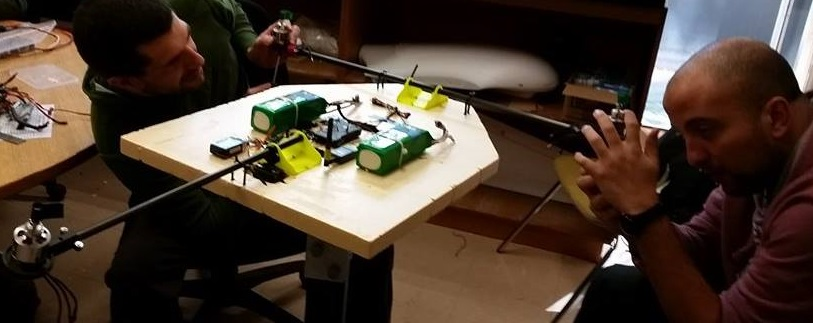
\includegraphics[width=200pt]{\IMAGEPATH /Prototype/scorpion}
	\caption{Prototype \#1: Scorpion }
	\label{fig:scorpion}
\end{figure}

\subsubsection*{Prototype \#2: ``Dragonfly''}
Once the proposed parts configuration had been tested, and the Scorpion had undergone some basic flight tests, the parts were moved onto the Skywalker X8. Some additional modifications were required such as rings for the front pole in between the layers of foam, and custom pole mounts. Table \ref{tab:tests} in Appendix \ref{sec:diary} shows major flight tests conducted on the Dragonfly prototype. A maximum hover time of 15 minutes has so far been achieved, with battery life still remaining after the flight.  

\begin{figure}[!ht]
	\centering
	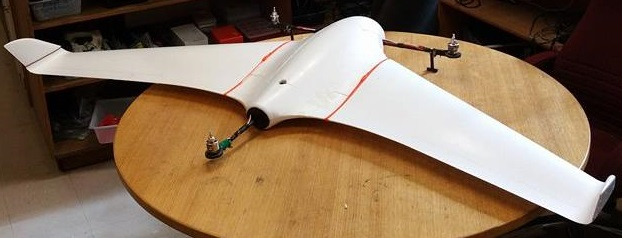
\includegraphics[width=200pt]{\IMAGEPATH /Prototype/dragonfly}
	\caption{Prototype \#2: Dragonfly }
	\label{fig:dragonfly}
\end{figure}

\subsection{Testing Platforms}
\subsubsection*{Thrust Testing}
In order to achieve the greatest lift for take-off, a number of tests were conducted on the thrust platform shown in Figure \ref{fig:rig} to measure the relative force of various propeller sizes and materials. The propellers were mounted on an arm, and the force generated by the motors at full throttle measured by a strain gauge.\\

Table \ref{tab:props} in Appendix \ref{sec:proptest} summarizes the results, which indicate that the 12$\times$6 APC (Plastic) blades produce the greatest force, and are best suited for take-off. Each propeller is able to pull over 2.02kg, for a total of 6kg of thrust from the 3 motors, which is more than enough for the craft, which is under 4kg, to take off.

\begin{figure}[!ht]
	\centering
	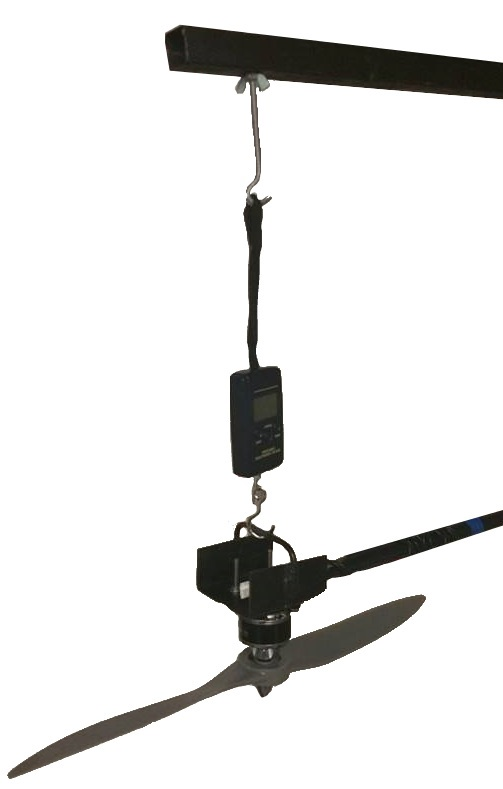
\includegraphics[width=160pt]{\IMAGEPATH /Prototype/rig}
	\caption{Thrust testing rig}
	\label{fig:rig}
\end{figure}

\subsubsection*{Balance Testing}
The balance table shown in Figure \ref{fig:balance_table} is able to freely rotate in 3 axes, and was used extensively to test the balance and performance of the UAV. By placing the UAV in the center of the table, parts could be shifted in order to move the center of mass to the desired location. The table was also used to test the UAV's ability to stabilize itself when subjected to disturbance.

\begin{figure}[!ht]
	\centering
	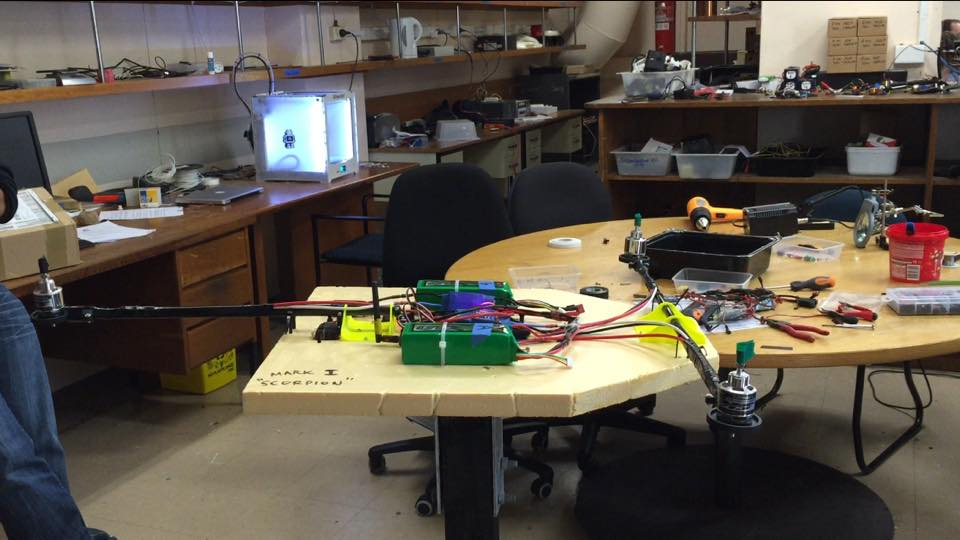
\includegraphics[width=200pt]{\IMAGEPATH /Prototype/balance_table}
	\caption{The Scorpion on the balance table}
	\label{fig:balance_table}
\end{figure}

\subsection{Iterative Design}
Through testing mechanisms and flight tests, a number of problems with the aircraft were tweaked and resolved. Table \ref{tab:tests} in Appendix \ref{sec:diary} shows the test flight dates, and item 62 in the project Gantt chart (Figure \ref{fig:gantt} in Appendix \ref{sec:gantt}) shows the large period of time taken up by repairs and additional testing. The sections below discuss some of these problems, test processes, and the resulting solutions.

\subsubsection*{Vibrations}
Numerous vibration related problems and set-backs were encountered during testing and evaluation of the prototypes. To combat this, an assortment of nyloc-nuts and spring-washers were utilized in order to fasten components together in a vibration resistant manner. The addition of four rubber ``feet'' to the base of each motor succeeded in damping any vibratory response down the pole shaft. Overall this was extremely effective in increasing stability, as vibrations appeared to be mitigated in follow-up tests.

\subsubsection*{3D Printing}
As previously mentioned, the 3D printed motor mounts underwent several design changes throughout the project, due to a number of problems with part strength, vibration and fastening of the mounts. A common problem was 3D printed parts fracturing during test flight, as a result of structural weakness.\\

The direction in which a design is 3D printed plays a vital role in where its strengths and weaknesses lie. Each print was orientated to maximise the strength of the layers against the most likely mode of failure from the forces and moments being applied. It was found that printing the layers on the same plane as both the bar and the direction of force gave the most strength, as the layer plane is in the same direction as the moment and they are not being pulled apart in any way.\\

Circular parts were also a significant issue. In order to achieve a ``true'' circle shape and thus lower friction for mated parts, critical ring shapes in designs were replaced by flatly printed ring inserts. These ring inserts were then either press fit into other printed components or ``merged'' onto other printed components using acetone. 
\todomessage{Alex/Wes: Give screenshot of example ring}

\subsubsection*{Gears}
Initially a 1:2 gear ratio was chosen for both front and back gear systems. Through testing however, it became evident that the torque provided by the servos was enough to overcome the friction and forces experienced during flight, so a 1:1 system which allowed for larger teeth and hence overall strength (shown in Table \ref{tab:minor}) was developed.

\subsubsection*{Wires and Soldering}
A major problem was that the high current passing through the electronics generated a significant amount of heat, resulting in soldered connections melting and power being disconnected from all systems. This was resolved by changing to non-lead based solder, increased melting temperatures by 40 degrees, ventilating the craft, and using higher spec wiring. 

\subsubsection*{Radio Failure}
Problems were encountered with the initial remote control transmitter leading to erratic, jerky behaviour during test flights. Range tests were conducted on the transmitter to determine its effective communication range. The transmitter is believed to be faulty, as its effective range was less than 5m, so the back up transmitter (HK-T6A V2) was chosen to resolved this problem.

\subsubsection*{Motor Failure}
During one flight test, a major failure caused one of the motors to burn out causing the aircraft to crash, resulting in several parts requiring repair. It is unknown whether this was caused due to manufacturing error in the motors, or debris short-circuiting the motor during flight. It was assumed the problem was caused by debris, and pre-flight checks now include a thorough clearing of potential debris from the area around the aircraft.

\subsubsection*{Power Module Failure}
The initial 3DR Power Module received with the PixHawk was faulty and a cheaper third party one was used for several flights. The UAV then began experiencing extremely unpredictable behaviour, which led to another major crash. After many sensor, current and voltage tests it was determined that the power module was the cause. A new 3DR Module was purchased, which has since been rendered unusable. A solution to the repeated power module failure has not been determined.